\section{Introduction}
In large scale (datacenter) networks, various networking challenges are confronted,
not only due to the complex topology that needs to be put in place, but
also because of the different networking services (Firewalls, NAT,...) required to
ensure a resilient network underlaying the datacenter’s servers. Further issues
arise which are mainly related to vendor lock-ins. In order to overcome these
shortcomings, a new form of networking functions was proposed, where they
are presented as an ordered set (chain) of basic service functions, increasing
therefore the flexibility of the networking functions and their adaptability to
the network’s changing requirements.\\
\section{Service Function Chains}
\textbf{\textcolor{blue}{\Large Definition}}\\
\\
SFC can be defined as a concept that enables the creation of composite
networking services (Service Functions) that are strictly oredered in order to
apply them to packets/frames matching the rules of these Service Functions
(Classification). SFC also offers a method of deployment for SFs, in which the
order of the service functions can be dynamically changed and independent of its
underlying topology using simply the exchanged\\
\\
\textbf{\textcolor{blue}{\Large Components}}\\
\\
\textbf{Service Function} A specific function that processes incoming packets following predefined rules. ctions can be involved in the delivery of added-value services. A non-exhaustive list of abstract service functions includes: firewalls, Deep Packet Inspection, NAT...\\
\\
\textbf{Service Function Forwarder} A logical component that forwards traffic to the connected
service functions according to information carried in the SFC
encapsulation. It does also handle traffic coming back from the
Service Functions.\\ 
\\
\textbf{Metadata} Exchanged context information among the different SFC components.\\
\\
\textbf{Service Function Path} a
constrained specification of where packets assigned to a certain
service function path must go. Specific details declaration is not mandatory. While in some cases the different Service Functions to be visited are fully specified, we can always maintain a certain level of abstraction in some other cases.\\
\\
\textbf{SFC Encapsulation} The SFC encapsulation  provides identification for SFP. It is equally  used by the SFC-aware functions. In addition, the SFC encapsulation carries metadata.\\
\\
\textbf{Rendered Service Path}  The different SFs and SFFs visited by a packet in the network.\\
\\
\textbf{SFC-Enabled Domain} A network or region of a network where SFC is implemented.\\
\\
\textbf{SFC Proxy} Logical component that removes and inserts SFC encapsulation on behalf of an     SFC-unaware service function.\\
\\
\textbf{\textcolor{blue}{\Large Architecture}}\\
\\
An SFC architecture does usually have to satisfy a set of principles in order to ensure using the SFC efficiently.\\
\\
\textbf{Topological Independence} 
The deployment SFs or SFCs does not require any changes in the underlay network forwarding topology.\\
\\
\textbf{Plane Separation} The packet handling operations should ne be confused with the the dynamic realization of the Service Forwarding Paths.\\
\\
\textbf{Classification} A specific SFP is responsible for any packet matching a specific rule.\\
\\
\textbf{Shared Metadata} Metadata/context data can be shared amongst Service Functions and classifiers, between SFs, and between external systems and SFs. Metadata could be used to provide and share the result of classification (that occurs within the SFC-enabled domain, or external to it) along an SFP.\\
\\ 
\textbf{Service Definition Independence} The SFC architecture does not depend on the details of SFs themselves.\\
\\
\textbf{SFC Independence} The creation, modification, or deletion of an SFC has no impact on other SFCs. The same is true for SFPs.\\
\\
\textbf{Heterogneous control/policy Points} The architecture allows SFs
to use independent mechanisms to
populate and resolve local policy and  local classification criteria.\\
\\
These architecture principles should be applied to the  different planes composing an SFC network. The environment associated to SFC is mainly separated into four main planes:\\
\\
\textbf{The Control Plane} mainly responsible for controlling and configuring the SFC related components. It should be noted that the control plane does only concern a subset of the parameters and facilities associated to the SF.\\
\\
\textbf{The Management Plane} it serves in allocating resources to the various SF and eventually active the various SF components. Management operations would consist in setting the number of CPU, memory bandwidth associated to the SFs as well as specific configuration parameters of the SFC components. Unlike the control plane, the management plane defines a large number of paramaters related to the SFC components configuration.\\
\\
\textbf{The Data Plane} consists in all SF components as well as the data exchanged between the SF components. Communications between SF components includes the packet themselves, their associated metadata, the routing logic or SF
logic. The SFC Data Plane can also be seen as all the elements that interact with a packet provided by an end user.\\
\\
\textbf{The SFC Tenant’s Users Data Plane} consists in the traffic data provided by the different users of the tenants. When a user is communicating with a server or another user, eventually from another administrative domain, the communication belongs to
the SFC Tenant’s Users Data Plane whenever packets are provided by the server or by the user.\\
\\
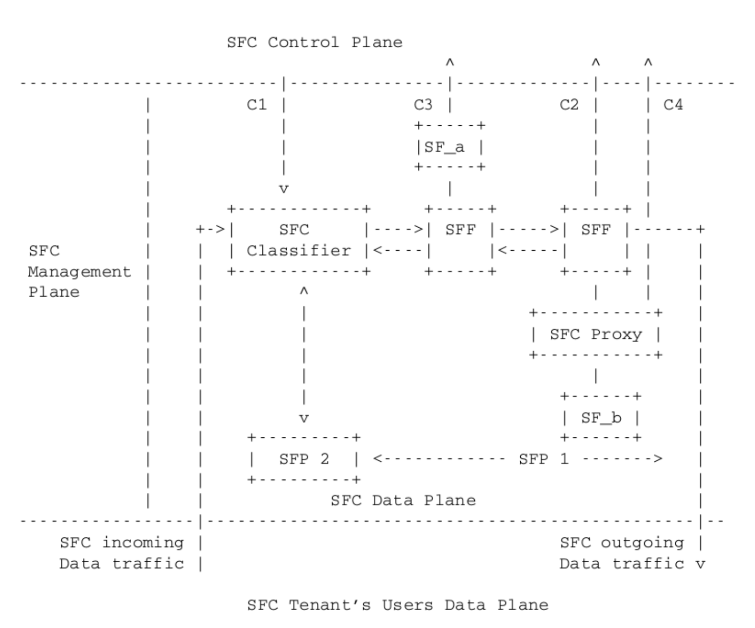
\includegraphics[scale=0.45]{sfc1}
\\
\\
\textbf{\textcolor{blue}{\Large SFC Security Concerns Overview}}\\
\\
The essential infrastructure required for the deployment of SFC is usually provided by a Cloud Provider. This infrastructure does include dedicated hardware serving a specified network function. The network function served by the dedicated hardware is the actual Service Function. If the SFC domain is not private to the company, the infrastructure and the dedicated hardwrare that it contains is often shared by multiple tenants. In some other cases, a local proxy does transparently redirect the local SFC network to an external SFC domain outside the local boundaries of the local infrastructure. Each SFC Tenant is responsible of its domain, that is to administrate or provision the necessary resource and control all its SFC element (e.g: defining SFC Paths, configuring the elements...). An SDN controller is responsible for the coordination of the SFC elements.\\
As for the security requirements for an SFC domain, thet aim to protect the deployed SFC architecture from attacks. Even in a private SFC deployment, where SFC components are considered to be in a trusted environment, inside attacks are still possible (e.g. inside attacker sniffing the SFC metadata, sending spoofed packets...). The evolution of the local architecture could require, at some point, interconnecting with a third party SF/SFF, which puts the initial domain basically outside of the local (private) domain. Multitenancy also does represent a security concern, due to the fact of sharing an SFC platform. Unless the tenants are strongly isolated (physically or logically), different networks may share a common SFF, and one tenant may update the SFP of the other tenant. Such misconfiguration has similar impact as a redirecting attack.\\
The threats in this work are analysed in each plane. Even if the architecture is divided into many planes, so that the interactions can be limited and controlled, but these interactions still exist and so may be used by an attacker. As a result, for each plane, the threat analysis is performed by analysing the vulnerabilities present within each plane, as well as those performed via the other planes. We focus mainly on the threats faced by the Data Plane.\\
Attacks may be performed from inside the SFC Data Plane or from outside the SFC Data plane. Therefore, the attacker is in at least one of the following planes: SFC Control Plane, SFC Management Plane or SFC Tenants’ Users Plane.\\
\\
\textbf{Attacks performed from the SFC Control Plane}
Vulnerabilites can be found basically in the interfaces used for communication between the SFC Control Plane and the SFC Data Plane. These interfaces are responsible for updating the classification rules for the SFC classifier, updating forwarding decisions for SFFs and updating SFs/SFC proxys internal state. An attacker may change the SFC Classifier classification and
completely modify the services provided by the SFC. This could result in avoiding control over the tenant's traffic.\\
\\
\textbf{Attacks performed from the SFC Management Plane}
This type of attacks are basically similar to the previous type, with the only difference being that the SFC Management Plan provides usually a greater control of the SFC component that the SFC Control Plane.\\
\\
\textbf{Attacks performed from the SFC Data Plane} Given that an attacker has taken control of an SFC component, various types of attacks can be performed, such as modification of the traffic, performing onpath attacks, generating additionnal traffic to create heavy load situations. On the other hand, The traffic within the SFC Data Plane is composed of multiple
layers: the transport layer, the SFC encapsulation layer and the SFC payload layer. As a result, attacker may use the traffic to perform attacks at various layers.\\
\\
\\
\textbf{1. Attacks performed at the transport layer}\\
Mainly related to the illegitimate SFC traffic that could be provided to the SF. A malicious node that is not expected to communicate with that SF may inject packets into the SFC, That may eventually spoof the IP address of legitimate SF, so the receiving SF may not be able to detect the packet is not legitimate.\\
\\
\textbf{2. Attacks performed at the SFC encapsulation/payload layer}\\
The SFC encapsulation and payload are considered as SF inputs. Therefore, attacks can be performed through them. Injecting malicious metadata in the encapsulation enveloppe may allow to inject traffic, due to the fact of escaping traffic authentication. When SFC traffic is not authenticated, an attacker may also modify on-path the packet. By changing some metadata contained in the SFC Encapsulation, the attacker may test and discover the logic of the SFF. Similarly, when the attacker is aware of the logic of a SFC component, the attacker may modify some metadata in order to modify the expected operation of the SFC.
\section{Blockchain Technology}
Blockchain has been initially introduced to the IT field as being the technology behind the digital currency Bitcoins. Nevertheless,  it is quickly being expanded to other fields (Health Care, Networking Security,..etc) after proving its worth in securing digital systems robustly. In this article, we take a look at the Bitcoins Blockchain model,  and the mechanisms used to prove the authenticity of digital transactions without the involvement of a trusted third-party.\\
\\
\textbf{\Large Problem of digital transactions}\\
\\
In principle, the third-party, which is usually a central bank, is involved in digital transactions to overcome the issue of double-spending: that is to say, to assure the authenticity of the buyer and the money that he owns. Since digital transactions are done over the internet, the money is being virtually transferred between business parties in file formats. If those files are being replicated and used quickly enough, an attacker can use the same money to do many transactions simultaneously.\\
\\
\\
\\
\textbf{\large How does Blockchain overcome double-spending ?}\\
\\
Firstly, Blockchain overcome the need for a third-party by making all the transactions public to all the participants in the system. Therefore, Blockchain is basically a distributed, peer to peer, database of blocks of transactions.  To assemble these blocks, transactions are being generated by timestamp servers. Once a block is assembled, a timestamp-hash is generated for the block.
\\
\\
\hspace*{-2cm}{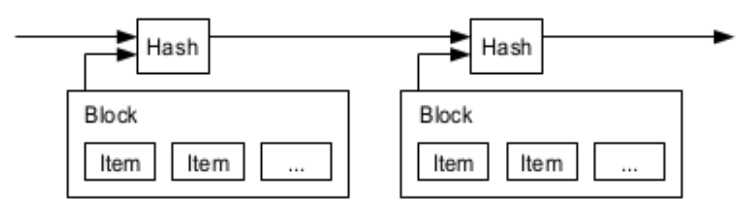
\includegraphics[scale=0.95]{bit1}}
\\
On the other hand, Blockchain is able to prove the authenticity of coins by tracking their records since their origin of generation, and that is achieved through the inclusion of previous block-hashes in the new block hash, hence the chain constitution.\\
Security and trust of the blockchain is further enhanced by the proof of work concept, which consists of scanning a value (nonce) that will generate a hash beginning a certain number of 0 bits.  the hash generated from this nonce value added to the hash coming from the previous block will result it the hash of the current block, that will be, again, delivered to the next block. Proof of work increase security by choosing the longest chain available as a reference for authenticity, meaning that the chain that has the most CPU power invested in it. Therefore, any attacker that wishes to gain access to the transactions data should assure that he can overpower the CPU capacity being in the chain, which can prove to be of extreme difficulty.
\\
\\
\hspace*{-1.7cm}{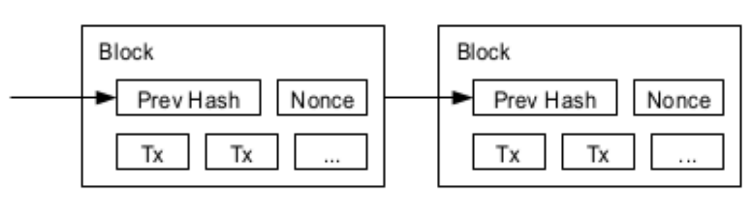
\includegraphics[scale=0.95]{bit2}}
\\
